\documentclass[xcolor=table]{beamer}

\usepackage[french]{babel}
\usepackage[latin1]{inputenc}
\usepackage[normalem]{ulem}
\usepackage[T1]{fontenc}
\usepackage{fancyhdr}   %% Pour la gestion des num�ros de page
\usepackage{graphicx}
\usepackage{amsmath}
\usepackage{mathrsfs}
\usepackage{amsfonts}
\usepackage{palatino}        %% Palatino fonts
\usepackage{mathptm}        %% PostScript Type 1 math fonts
\usepackage{dsfont} %% Pour mathds
\usepackage{color}
%%\usepackage{pstricks}
\usepackage{xmpmulti}
\usepackage{hyperref}
\usepackage{multimedia}
\usepackage{multirow}
%\usepackage[table]{xcolor}
\usepackage{fourier-orns}
\usepackage{subfigure}
\usepackage{tikz}

\DeclareMathAlphabet{\mathpzc}{OT1}{pzc}{m}{it}

\definecolor{vert}{rgb}{0.07,0.7,0.00}
\definecolor{gris}{gray}{0.70}
\definecolor{gris2}{gray}{0.95}
\definecolor{bleu}{rgb}{0.19,0.19,0.68}

%table setting
\newcommand\T{\rule{0pt}{2.6ex}}
\newcommand\B{\rule[-1.2ex]{0pt}{0pt}}
\renewcommand{\thesubfigure}{\thefigure.\arabic{subfigure}}

\usetheme{allee_marine} %voir fichier beaerthemeallee_marine.sty   ==> \usetheme{allee_marine}


%%%%%%%%%%%%%%%%%%%%%%%%%% Pr�sentation du document %%%%%%%%%%%%%%%%%%%%%%%%%%
\title[Master 1 Project]{Indexing big colored image bank : Texture 3.0}
\author[Etienne CAILLAUD, Thomas LE BRIS, Ibrahima GUEYE, Gaetan ADIER]{\textbf{Etienne CAILLAUD, Thomas LE BRIS, Ibrahima GUEYE, Gaetan ADIER}}
\institute [XLIM-SIC UMR CNRS 7252]{\textbf{XLIM-SIC Laboratory UMR CNRS 7252, Poitiers, France}}
\date{}

%%%%%%%%%%%%%%%%%%%%%%% Num�ro de pages en bas � gauche %%%%%%%%%%%%%%%%%%%%%%
\addtobeamertemplate{footline}{\color{blue}\hfill\insertframenumber/\inserttotalframenumber}

\pgfdeclareimage[height=96mm,width=128mm]{nombidon}{mood_eye_light}
\setbeamertemplate{background}{\pgfuseimage{nombidon}}

\pgfdeclareimage[height=96mm,width=128mm]{nombidon2}{mood_eye_light}
\setbeamertemplate{background}{\pgfuseimage{nombidon2}}

%%----------------------------------------------------------------------------
%% A chaque d�but de sous-section : g�n�re une table des mati�res
%%----------------------------------------------------------------------------
\AtBeginSection[]
{
   \setbeamertemplate{background}{\pgfuseimage{nombidon}}
   \begin{frame}<beamer>
    \frametitle{Outline}
    \tableofcontents[currentsection, hideallsubsections] %% affiche la section courante et les autres en gris�, masque les sous-sections
   \end{frame}
  \setbeamertemplate{background}{\pgfuseimage{nombidon2}}
}

\AtBeginSubsection[]
{
  \setbeamertemplate{background}{\pgfuseimage{nombidon}}
  \begin{frame}<beamer>
    \tableofcontents[sectionstyle=show/shaded,subsectionstyle=show/shaded/hide, subsubsectionstyle =hide]
  \end{frame}
   \setbeamertemplate{background}{\pgfuseimage{nombidon2}}
}

\AtBeginSubsubsection[]
{
  \setbeamertemplate{background}{\pgfuseimage{nombidon}}
  \begin{frame}<beamer>
    \tableofcontents[sectionstyle=show/shaded,subsectionstyle=show/shaded/hide,subsubsectionstyle =show/shaded/hide]
  \end{frame}
   \setbeamertemplate{background}{\pgfuseimage{nombidon2}}
}


%%%%%%%%%%%%%%%%%%%%%%%%%%%%%%%%%%%%%%%%%%%%%%%%%%%%%%%%%%%%%%%%%%%%%%%%%%%%%%
%%%%%%%%%%%%%%%%%%%%%%%%%%%%                       %%%%%%%%%%%%%%%%%%%%%%%%%%%
%%%%%%%%%%%%%%%%%%%%%%%%%%     D�BUT DU DOCUMENT     %%%%%%%%%%%%%%%%%%%%%%%%%
%%%%%%%%%%%%%%%%%%%%%%%%%%%%                       %%%%%%%%%%%%%%%%%%%%%%%%%%%
%%%%%%%%%%%%%%%%%%%%%%%%%%%%%%%%%%%%%%%%%%%%%%%%%%%%%%%%%%%%%%%%%%%%%%%%%%%%%%
\begin{document}
\graphicspath{{images/}}
\setbeamercolor{block title example}{bg = gray}

\begin{frame}
    \vspace{-1.5cm}
    \begin{tikzpicture}[remember picture,overlay]
        \node[xshift=0cm, above=8.6cm] at (current page.south west)
        {
\includegraphics[width=40cm,height=0.9cm]{cache_titre.png}};
        \node[xshift=2cm, above=2.8cm] at (current page.south west)
        {
\includegraphics[height=1.5cm]{Xlim.png}};
        \node[xshift=11cm, above=3cm] at (current page.south west)
        {
\includegraphics[height=1cm]{logo_une.jpg}};
        \node[xshift=6.5cm, above=0.7cm] at (current page.south west)
        {
\includegraphics[height=1.6cm]{Lifeclef.png}};
    \end{tikzpicture}
    \titlepage
\end{frame}

%%%%%%%%%%%%%%%%%%%%%%%%%%%%%%%%%%%%%%%%%%%%%%%%%%%%%%%%%%%%%%%%%%%%%%%%%%%%%%%%%%%%%%%%%%%%%%%%%%%%%
%%%%%%%%%%%                        D�but de la pr�sentation                       			 %%%%%%%%
%%%%%%%%%%%%%%%%%%%%%%%%%%%%%%%%%%%%%%%%%%%%%%%%%%%%%%%%%%%%%%%%%%%%%%%%%%%%%%%%%%%%%%%%%%%%%%%%%%%%%
\section{Introduction}
%%-----------------------------------------------------------------------------------------
%%-----------------------------------------------------------------------------------------
\begin{frame} \frametitle{Image Indexing}
%%-----------------------------------------------------------------------------------------
   \begin{figure}[h]
        \centering
        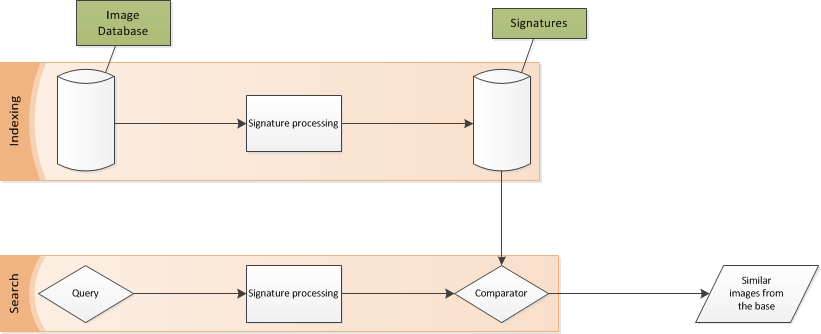
\includegraphics[scale=0.35]{ImgIndx.png}
        \caption{Online image indexing}
        \label{fig:img_index}
    \end{figure}
\end{frame}

%%-----------------------------------------------------------------------------------------

\begin{frame} \frametitle{Descriptor}
%%-----------------------------------------------------------------------------------------
    \begin{figure}[h]
        \centering
        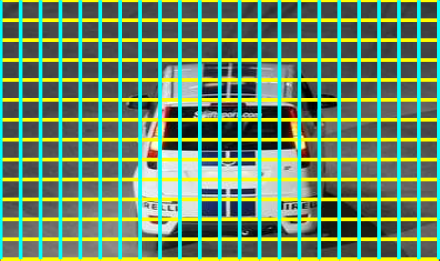
\includegraphics[scale=0.35]{dense_grid.png}
        \caption{Dense grid keypoints}
        \label{fig:img_densegrid}
    \end{figure}

\end{frame}
%%-----------------------------------------------------------------------------------------

\begin{frame} \frametitle{Descriptor}
%%-----------------------------------------------------------------------------------------
    \begin{figure}[h]
        \centering
        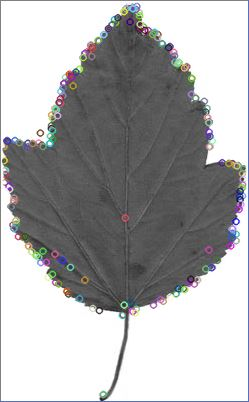
\includegraphics[scale=0.35]{siftKP.jpg}
        \caption{Points of interest keypoints}
        \label{fig:img_poi}
    \end{figure}

\end{frame}
%%-----------------------------------------------------------------------------------------


\section{Team presentation}

\begin{frame} \frametitle{Deadlines}
%XLIM-SIC Laboratory of University of Poitiers
%\begin{itemize}
%\item Noel Richard ( Researcher in Color images): Supervisor
%\item David Helbert ( Researcher in Signal-Image-Communications): Supervisor
%\item Thierry Urruty ( Researcher in Color images): Customer
%\end{itemize}
\begin{figure}[h]
    \center
    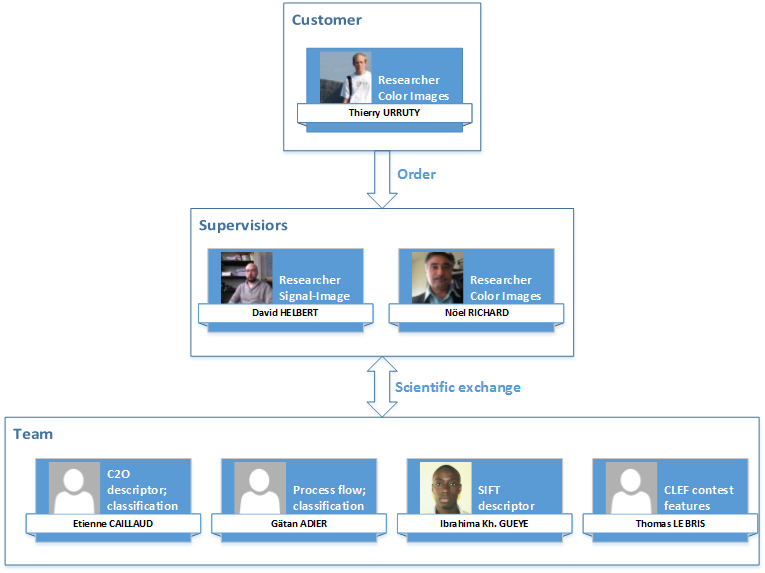
\includegraphics[scale=0.5]{Dessin1.png}
    \caption{Team}\label{fig:team}
\end{figure}

\end{frame}
%%-----------------------------------------------------------------------------------------

\section{User requirement}
\begin{frame} \frametitle{Software}
\begin{itemize}
 \item Design  software programs:\\
   indexation of  images database,calculate descriptor according to  nature images
\item Adapt the last up to date designed color and texture attributes to the current image classification
\item Compare our results (using CLEF challenge metrics)
\item Provide an abstract of the comparisons and a technical report
\end{itemize}






%%-----------------------------------------------------------------------------------------
\end{frame}
%%-----------------------------------------------------------------------------------------

\section{Work achievement}
%%-----------------------------------------------------------------------------------------
\begin{frame} \frametitle{SIFT(Scale-Invariant Feature Transform)}

Key-points detection (x,y,$\sigma$)
\begin{itemize}

\item Scale-space extrema detection\\


 \item  Key-point location\\


\item Orientation assignment\\


\item key-point descriptor 
\\

\end{itemize}
\end{frame}

\begin{frame} \frametitle{SIFT(Scale-Invariant Feature Transform)}
\begin{figure}[htbp]
    \begin{minipage}[c]{.45\linewidth}
      \begin{center}
	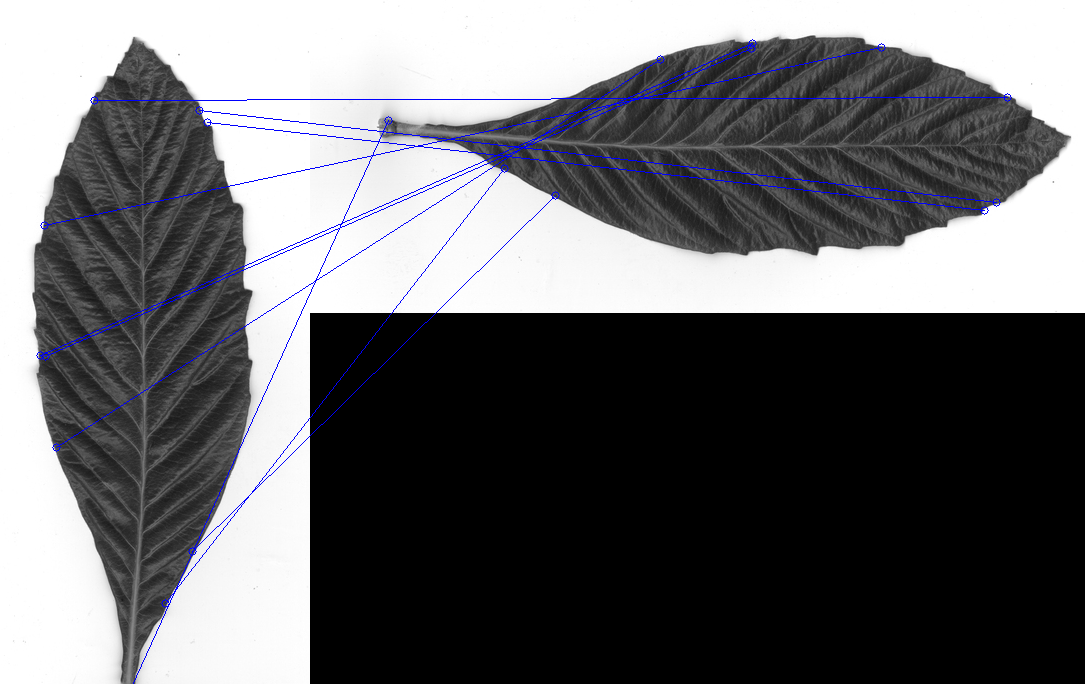
\includegraphics[scale=0.20]{Capture1.png}
	\caption{SIFT test1}
	\label{figure:Illustration}
      \end{center}
    \end{minipage}
    \hfill
    \begin{minipage}[c]{.45\linewidth}
      \begin{center}
	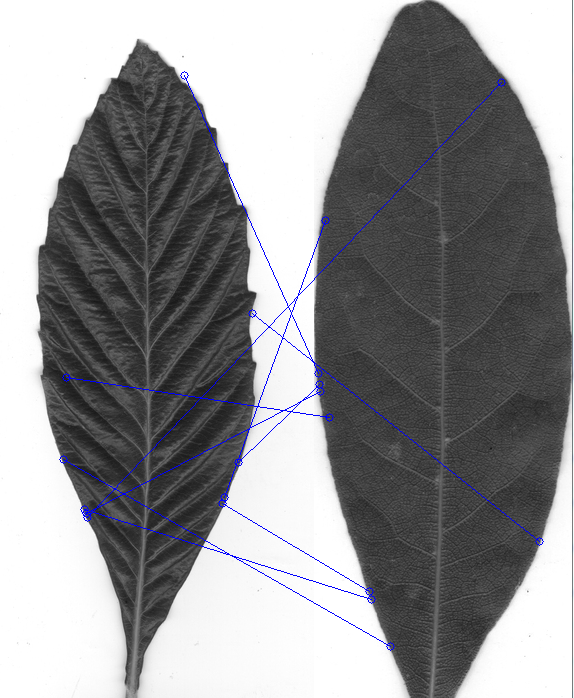
\includegraphics[scale=0.20]{Capture.png}
	\caption{SIFT test2}
	\label{figure:Illustration}
      \end{center}
    \end{minipage}
  \end{figure}
\end{frame}
%%-----------------------------------------------------------------------------------------
\begin{frame}\frametitle{C$_2$O(1/3)}

- The C$_2$O matrix

\begin{itemize}
\item Conversion to $L^* a^* b^*$ space
\item C$_2$O matrix calculation.
\item C$_2$O signature extraction.
\end{itemize}


\end{frame}


\begin{frame}\frametitle{C$_2$O(2/3)}

- The C$_2$O matrix

\begin{itemize}
\item<1-> The color difference computation (in the $L^* a^* b^*$ space).
\only<1> {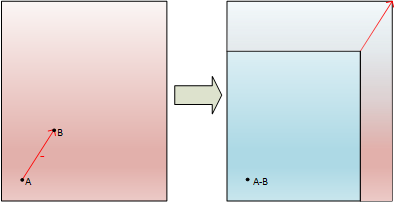
\includegraphics[height=4cm]{ColorDiff.png}} % Changer l'image
\item<2-> The C$_2$O matrix in a 3-D repository.
\only<2> {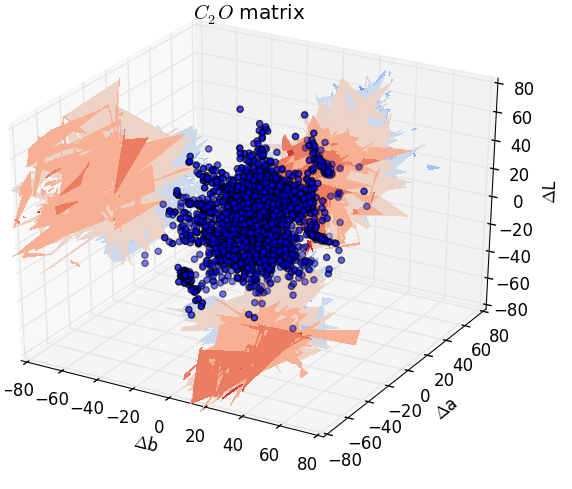
\includegraphics[height=4cm]{C2OMatrix.png}}
\end{itemize}


\end{frame}

\begin{frame}\frametitle{C$_2$O(3/3)}

- The C$_2$O feature extraction

\begin{itemize}
\item<1-> Spherical from cartesian repository.
\only<1> {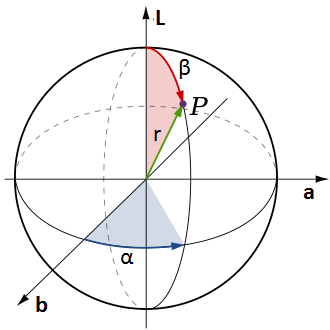
\includegraphics[height=5cm]{Spherical_Coordinates.png}} % Changer l'image
\item<2-> Quantization for one $\beta$ interval.
\only<2> {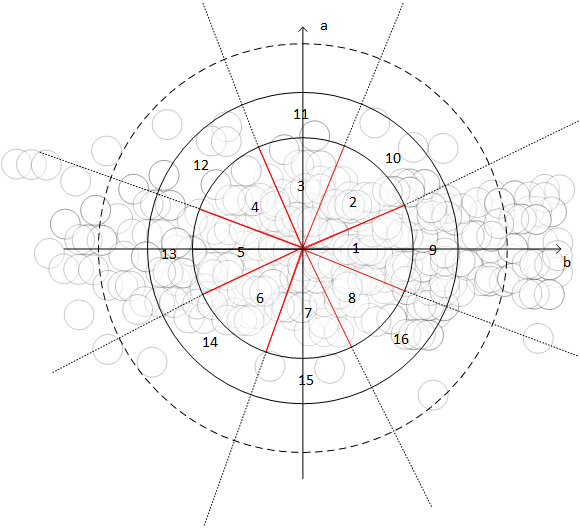
\includegraphics[height=5cm]{QuantificationSphericToHist1.png}}
\item<3-> Histogram obtained for one $\beta$ interval.
\only<3> {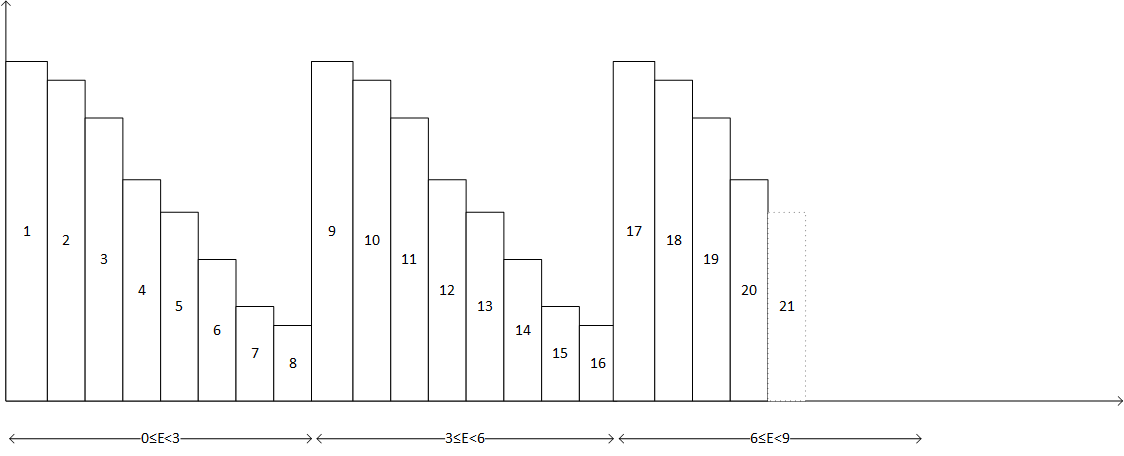
\includegraphics[height=4cm]{QuantificationSphericToHist2.png}}
\item<4-> Quantization for each $\beta$ interval.
\only<4> {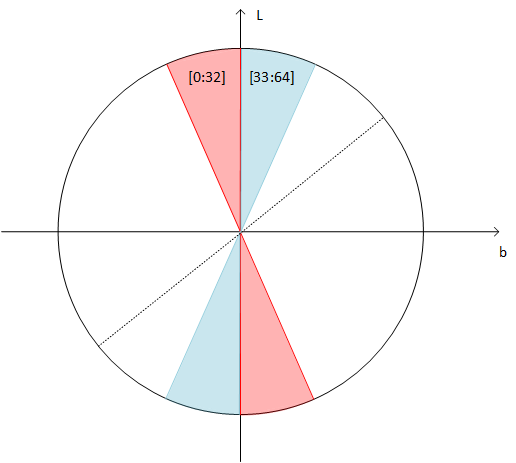
\includegraphics[height=5cm]{QuantificationSphericToHist3.png}}
\item<5-> Final signature obtained.
\only<5> {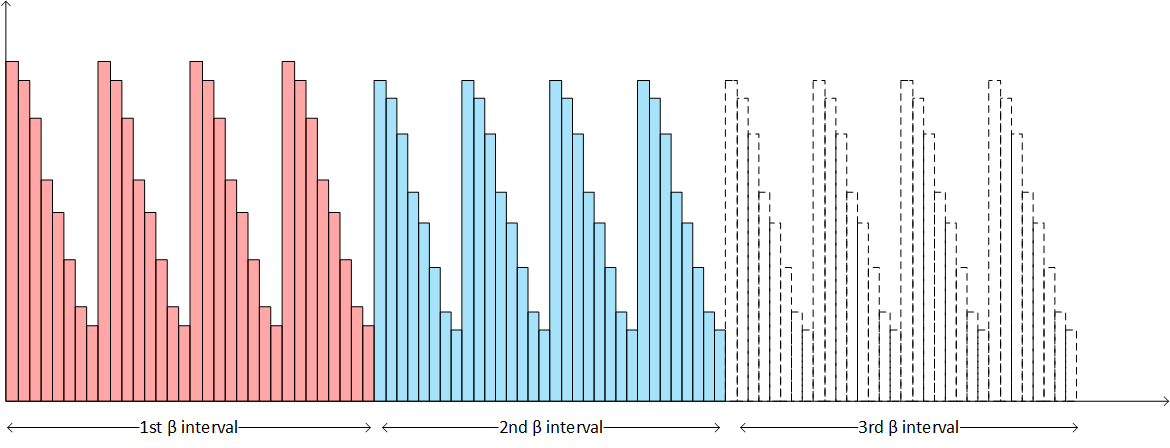
\includegraphics[height=3.5cm]{QuantificationSphericToHist4.png}}

\end{itemize}


\end{frame}

%%-----------------------------------------------------------------------------------------

\begin{frame} \frametitle{Classification (Bag of words)}
Reducing the number of points.

\begin{figure}[htbp]
    \begin{minipage}[c]{.55\linewidth}
      \begin{center}
        \begin{itemize}
            \item K-means
            \begin{itemize}
                \item Attribute the vectors to centroid vectors.
            \end{itemize}
        \end{itemize}
      \end{center}
    \end{minipage}
    \hfill
    \begin{minipage}[c]{.40\linewidth}
      \begin{center}
    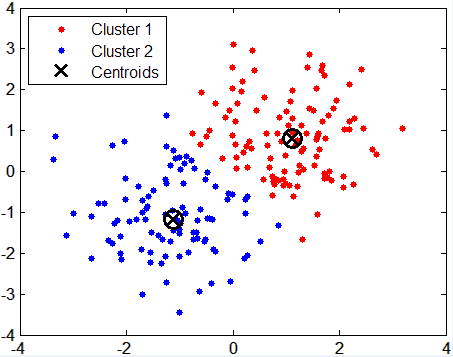
\includegraphics[scale=0.20]{kmeans.png}
    \caption{K-means}
    \label{fig:kmeans}
      \end{center}
    \end{minipage}
\end{figure}

\begin{figure}[htbp]
    \begin{minipage}[c]{.40\linewidth}
      \begin{center}
    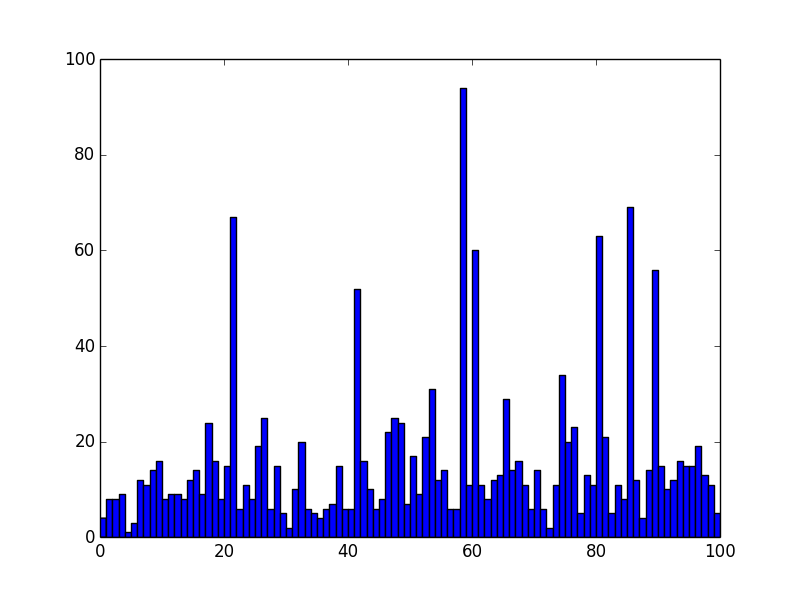
\includegraphics[scale=0.18]{132_sig.png}
    \caption{Signature}
    \label{fig:Sig}
      \end{center}
    \end{minipage}
    \hfill
    \begin{minipage}[c]{.55\linewidth}
      \begin{center}
        \begin{itemize}
            \item Signature
            \begin{itemize}
                \item Design histogram in function of assignment of the vectors.
            \end{itemize}
        \end{itemize}
      \end{center}
    \end{minipage}
\end{figure}


\end{frame}


\begin{frame}\frametitle{Classification (K-nn(1/2))}

- The k nearest neighbor method

\begin{itemize}
\item<1-> Comparison to the dictionary .
\only<1> {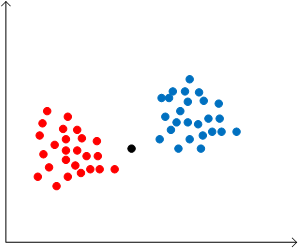
\includegraphics[height=4.2cm]{knnwc.png}} % Changer l'image
\only<2> {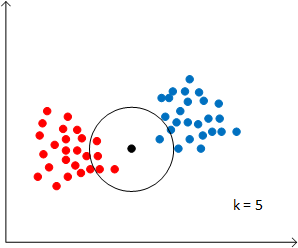
\includegraphics[height=4cm]{knnac.png}
\newline - 4 Occurrences of the 'red' class , - 1 occurrence of the 'blue' class \newline - The new point is attributed to the 'red' class}
\end{itemize}

\end{frame}

\begin{frame}\frametitle{Classification (K-nn(1/2))}

- Application for image classification

\begin{itemize}
\item More complex data.
\item Distances on signature vectors extracted from the K-mean method.
\item One most adapted distance type for each descriptor .
\end{itemize}

\end{frame}


%%-----------------------------------------------------------------------------------------


\begin{frame} \frametitle{CLEF}
%%-----------------------------------------------------------------------------------------
   \begin{itemize}
		\item What is CLEF ?
	    \item What did we gained from enrolling ?
		\begin{figure}[h]
			\centering
			\includegraphics[scale=0.35]{oneprunus.png}
			\caption{Points of interest keypoints}
			\label{fig:img_obsID}
		
		\end{figure}
		\item benchmark
	\end{itemize}
\end{frame}
%%-----------------------------------------------------------------------------------------


\begin{frame} \frametitle{Process flow}

\begin{itemize}
    \item Main function which control all the process
    \begin{itemize}
        \item Create the tree structure.
        \item Allows the choice of descriptors.
    \end{itemize}
\end{itemize}

\begin{figure}[h]
        \centering
        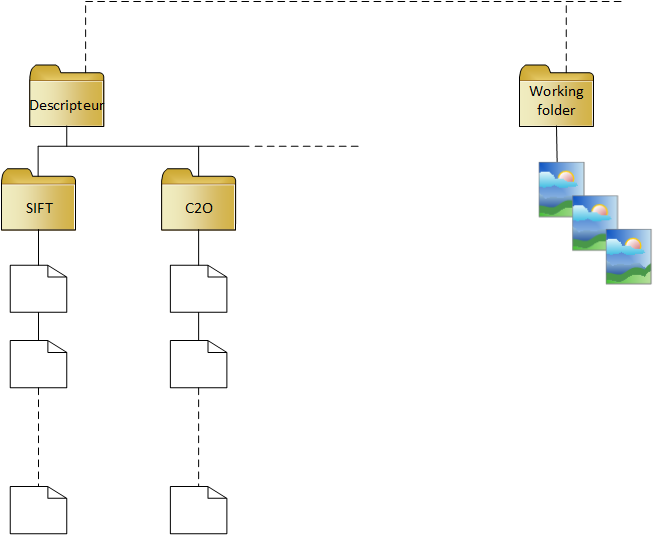
\includegraphics[scale=0.25]{arborescence.png}
        \caption{Tree structure}
        \label{fig:img_arbo}
    \end{figure}


\end{frame}
%%-----------------------------------------------------------------------------------------

\section{Results and Discussion}
\begin{frame} \frametitle{Results}
%%-----------------------------------------------------------------------------------------
\begin{itemize}
    \item Reduce data-base of 100 images composed of only 4 species.
    \item Compare the two descriptors SIFT and C$_2$O.
\end{itemize}

\begin{figure}[htbp]
    \resizebox{3.5cm}{!}{
    \begin{minipage}[c]{.55\linewidth}
      \begin{center}
        \begin{table}[H]
        \centering
        \caption{SIFT result}
        \label{tab1}
        \begin{tabular}{|l|l|l|l|l|}
        \hline
        ID & Training Base & Test Base & Correct & Accuracy \\ \hline
        173 & 17 & 8 & 4 & 50\% \\ \hline
        1102 & 22 & 3 & 1 & 33\% \\ \hline
        1889 & 16 & 9 & 1 & 11\% \\ \hline
        2717 & 15 & 10 & 7 & 70\% \\ \hline
        Total & 70 & 30 & 9 & / \\ \hline
        \end{tabular}
        \end{table}
      \end{center}
    \end{minipage}}

    \resizebox{3.5cm}{!}{
    \begin{minipage}[c]{.55\linewidth}
      \begin{center}
            \begin{table}[H]
            \caption{C$_2$O result}
            \label{tab2}
            \begin{tabular}{|l|l|l|l|l|}
            \hline
            ID & Training Base & Test Base & Correct & Accuracy \\ \hline
            173 & 17 & 8 & 1 & 12.5\% \\ \hline
            1102 & 22 & 3 & 1 & 33\% \\ \hline
            1889 & 16 & 9 & 0 & 0\% \\ \hline
            2717 & 15 & 10 & 7 & 70\% \\ \hline
            Total & 70 & 30 & 9 & / \\ \hline
            \end{tabular}
            \end{table}
      \end{center}
    \end{minipage}}
\end{figure}

\end{frame}
%%-----------------------------------------------------------------------------------------

\begin{frame} \frametitle{Discussion}

\begin{itemize}
    \item Classification
    \vspace{0.3cm}
    \begin{itemize}
        \item To much reducing on the K-means (100 words).
        \vspace{0.15cm}
        \item Euclidean distance not the most efficient or adapt.
    \end{itemize}
    \vspace{0.7cm}
    \item C$_2$O
    \vspace{0.3cm}
    \begin{itemize}
        \item The concatenation way is not optimal.
    \end{itemize}
\end{itemize}
\end{frame}
%%-----------------------------------------------------------------------------------------

\section{Project Management}
\begin{frame}\frametitle{Project management (1/2)}

- The scrum methodology

\begin{itemize}
\item One sprint per week.
\item Daily scrum meeting.
\item Complete time repartition on the product backlog.

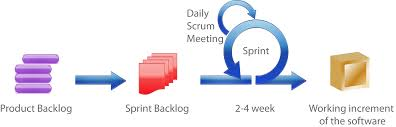
\includegraphics[height=2cm]{scrum.jpg}
\end{itemize}

\end{frame}


\begin{frame}\frametitle{Project management (2/2)}

- The sprint backlog : Trello board

\begin{itemize}

\item<1-> Progress on one sprint.\vspace{0.5cm}
\only<1> {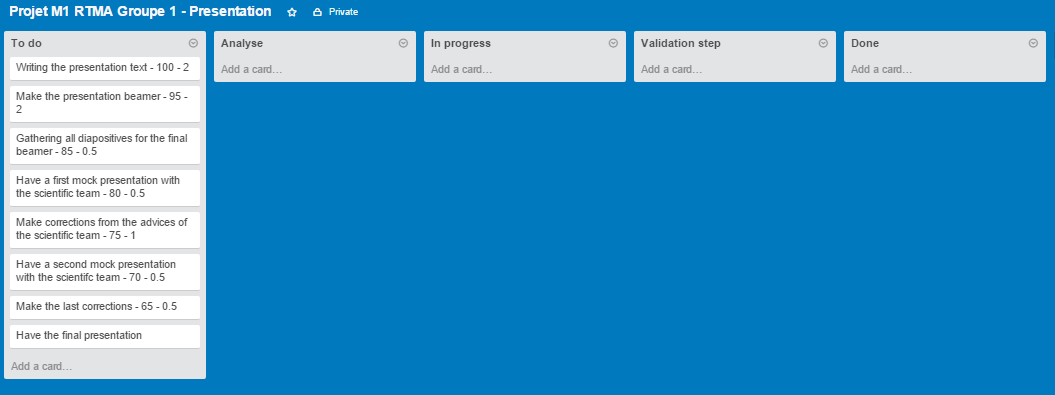
\includegraphics[height=3.7cm]{trello1.png}} % Changer l'image
\only<2> {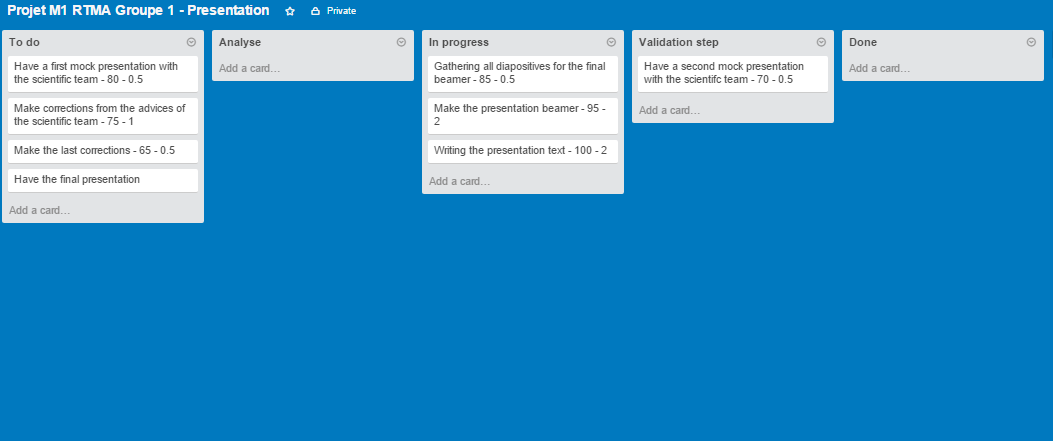
\includegraphics[height=4cm]{trello2.png}}
\only<3> {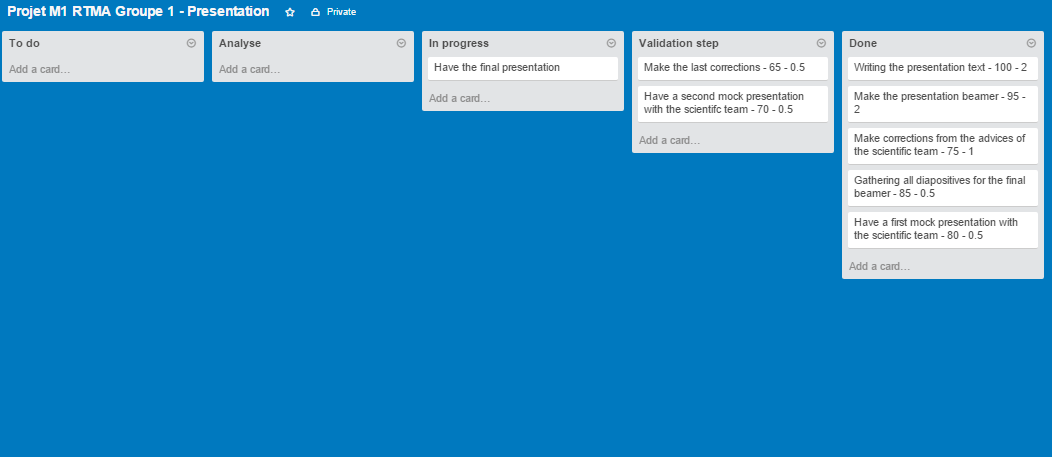
\includegraphics[height=4cm]{trello3.png}}
\end{itemize}

\end{frame}
%%-----------------------------------------------------------------------------------------

\section{Conclusion}
\begin{frame}\frametitle{Conclusion}
%%-----------------------------------------------------------------------------------------
   \begin{itemize}
        \item Things we learned
        \item Errors/Perspectives
    \end{itemize}

\end{frame}
%%-----------------------------------------------------------------------------------------


\section{}
\begin{frame}\frametitle{}
%%-----------------------------------------------------------------------------------------
    \begin{center}
        Thanks for attention
    \end{center}
\end{frame}
%%-----------------------------------------------------------------------------------------


\end{document}

